\begin{observation}
\ \begin{center}
\begin{minipage}{.48\textwidth}
		\adjustbox{scale=.7, center}{
			\begin{tikzcd}
				&  &  & \text{Relation} \arrow[ddddd, "\text{Left-Total}", bend left] \arrow[ddddd, "\text{Many-to-one}"', bend right] &  &  &\\
				&  &  & &  &  &   \\
				&  &  & &  &  &  \\
				&  &  &  &  &  &  \\
				&  &  & &  &  &  \\
				&  &  & \text{Function} \arrow[rrrddd, "\text{Right-Total}"] \arrow[lllddd, "\text{One-to-Many}"']                             &  &  &  \\
				&  &  &  &  &  & \\
				&  &  & &  &  &   \\
				\text{Injection} \arrow[rrrdd] &  &  &   &  &  & \text{Surjection} \arrow[llldd] \\
				&  &  &  &  &  &  \\&  &  & \text{Bijection} &  &  &              
		\end{tikzcd}}
\end{minipage}\quad
\begin{minipage}{.48\textwidth}
		\adjustbox{scale=.7, center}{
			\begin{tikzcd}
				&  &  & f\subseteq S\times T \arrow[ddddd, "\displaystyle\frac{s\in S}{\exists t\in T\ \text{s.t.}\ s\mathrel{f}t}", bend left] \arrow[ddddd, "\displaystyle\frac{s\mathrel{f}t_1\quad s\mathrel{f}t_2}{t_1=t_2}"', bend right] &  &  &\\
				&  &  & &  &  &   \\
				&  &  & &  &  &  \\
				&  &  &  &  &  &  \\
				&  &  & &  &  &  \\
				&  &  & S\overset{f}{\to} T \arrow[rrrddd, "\displaystyle\frac{t\in T}{\exists s\in S\ \text{s.t.}\ t\mathrel{f}s}"] \arrow[lllddd, "\displaystyle\frac{s_1\mathrel{f}t\quad s_2\mathrel{f}t}{s_1=s_2}"']                             &  &  &  \\
				&  &  &  &  &  & \\
				&  &  & &  &  &   \\
				S\overset{f}{\rightarrowtail} T \arrow[rrrdd] &  &  &   &  &  & S\overset{f}{\twoheadrightarrow} T \arrow[llldd] \\
				&  &  &  &  &  &  \\&  &  & S\overset{f}{\leftrightarrow} T &  &  &              
		\end{tikzcd}}
\end{minipage}
\end{center} 

\begin{center}\adjustbox{scale=.7}{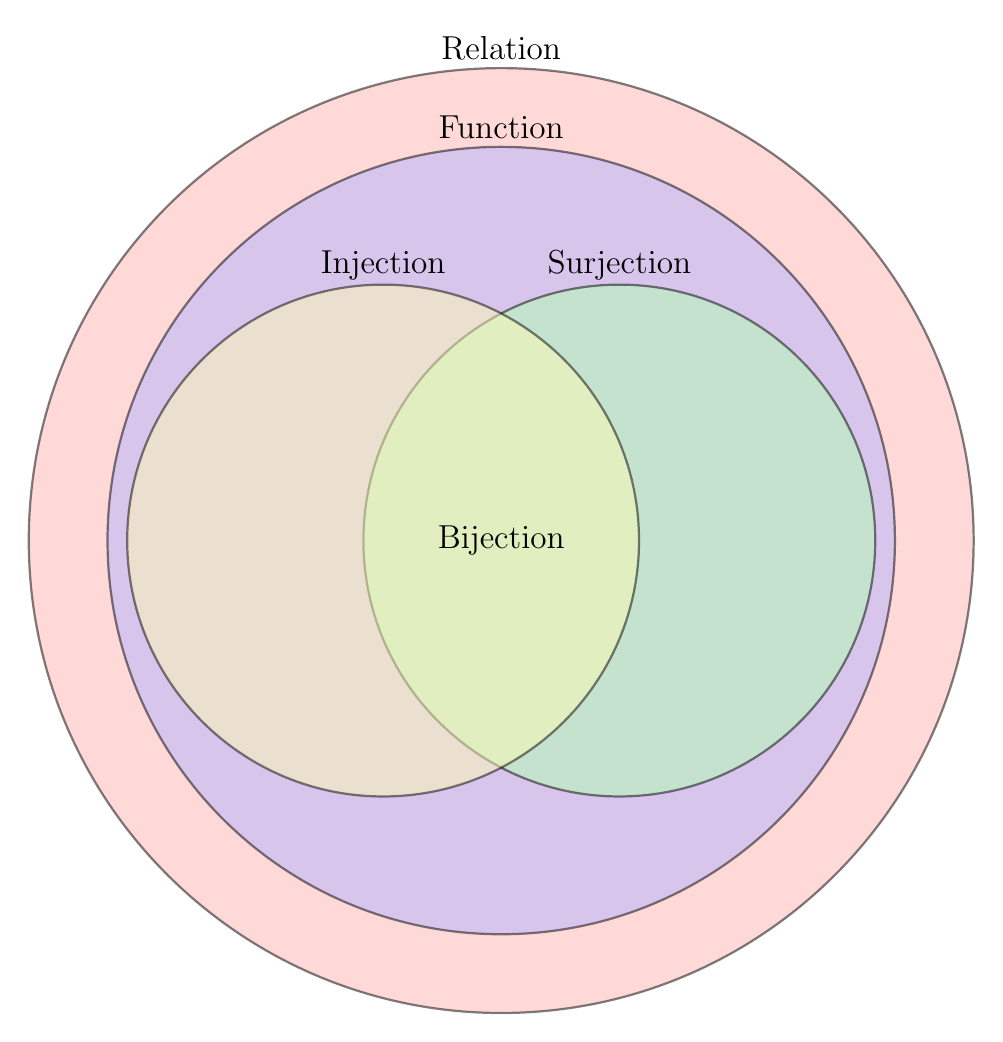
\begin{tikzpicture}
% Define circles
\draw[thick, fill=red!30, opacity=0.5] (0,0) circle (6cm); \node at (0, 6.25) {\large Relation};
\draw[thick, fill=blue!30, opacity=0.5] (0,0) circle (5cm); \node at (0, 5.25) {\large Function};
\draw[thick, fill=green!30, opacity=0.5] (1.5,0) circle (3.25cm); \node at (1.5, 3.5) {\large Surjection};
\draw[thick, fill=yellow!30, opacity=0.5] (-1.5,0) circle (3.25cm); \node at (-1.5, 3.5) {\large Injection};
%\draw[thick, fill=violet!30, opacity=0.5] (0,0) circle (1cm); 
\node at (0, 0) {\large Bijection};
\end{tikzpicture}}
\end{center}
\end{observation}

\section{Functions}
\defbox[Function]{
\begin{definition}
	Let $S$ and $T$ be sets. A \textbf{function} $f$ \textbf{from $\boldmath{S}$ to $\boldmath{T}$} is a relation on $S\times T$ satisfying as follows: \begin{enumerate}[(i)]
		\item (\textbf{Left-Total}\footnote{Every element of $S$ relates to some element of $T$.}) $\dom f=S$, \ie, \[
		s\in S\implies \exists t\in T:f(s)=t.
		\]
		\item (\textbf{Many-to-one}\footnote{Every element of $\dom{f}$ relates to no more than one element of its $\cdm{f}$.}) Let $s\in\dom{f}$ and $t_1,t_2\in\cdm{f}$. Then \[
		f(s)=t_1\land f(s)=t_2\implies s_1=s_2.
		\]
	\end{enumerate}
\end{definition}
}

\defbox[Domain, Codomain, and Range]{
\begin{definition}
\ \begin{itemize}
	\item \textbf{Domain:} The domain of a function \( f: A \to B \) is the set \( A \) of all possible input values for which the function is defined. Formally:
	\[
	\text{Domain}(f) = A
	\]
	\item \textbf{Co-domain:} The co-domain of a function \( f: A \to B \) is the set \( B \) which includes all potential output values. It is the target set for the function. Formally:
	\[
	\text{Co-domain}(f) = B
	\]
	\item \textbf{Range:} The range (or image) of a function \( f \) is the set of all actual output values produced by the function. It is a subset of the co-domain \( B \). Formally:
	\[
	\text{Range}(f) = f[A] = \{ f(a) \mid a \in A \} \subseteq B
	\]
\end{itemize}
\end{definition}
}
\begin{remark}
\ \\ \adjustbox{scale=.9, center}{
\begin{tikzpicture}
	% Draw the sets A and B
	\draw[thick] (-3,0) ellipse (2 and 3);
	\draw[thick] (3,0) ellipse (2 and 3);
	
	% Labels for sets
	\node at (-3, 3.25) {$\dom f$};
	\node at (3, 3.25) {$\cdm f$};
	
	% Draw the arrows representing the function
	\draw[-Stealth] (-2, 3.25) -- (2,3.25) node[midway, above] {$f$};
	\draw[thick, dotted] (-3,3) -- (3,1.5);
	\draw[thick, dotted] (-3,-3) -- (3,-1.5);
	
	\draw[fill] (-2.5,0) circle (.1);
	\draw[fill] (2.5,0) circle (.1);
	\draw[|-Stealth, line width=.5mm] (-2.25, 0) -- (2.25, 0);
	
	% Labels for elements in Domain
	\node at (-3, 0) {$a$};
	
	% Labels for elements in Co-domain
	\node at (3, 0) {$f(a)$};
	
	% Highlight the range
	\draw[thick, dotted] (3, 0) ellipse (1 and 1.5);
	
	% Label for the range
	\node at (3, 1.75) {$f[A]$};
\end{tikzpicture}}
\end{remark}

\section{Composition}
\defbox[Composition of Functions]{
\begin{definition}
Given two functions \( f \) and \( g \), where \( f: A \to B \) and \( g: B \to C \), the \textbf{composition} of \( g \) and \( f \), denoted by \( g \circ f \), is a function from \( A \) to \( C \) defined as follows:
\[
(g \circ f)(x) = g(f(x))
\]
for all \( x \in A \). That is, \[
\fullfunction{g\circ f}{A}{C}{a}{(g\circ f)(a)}
\]
\end{definition}}
\begin{remark}
\ \begin{itemize}
	\item \textbf{Functions}:
	\begin{itemize}
		\item Let \( f: B \to C \) be a function from set \( B \) to set \( C \).
		\item Let \( g: A \to B \) be a function from set \( A \) to set \( B \).
	\end{itemize}
	
	\item \textbf{Composition Definition}:
	\begin{itemize}
		\item The composition \( f \circ g \) is a function from \( A \) to \( C \).
		\item For each \( x \in A \), \( (f \circ g)(x) \) is defined as \( f(g(x)) \).
	\end{itemize}
	
	\item \textbf{Domain and Range}:
	\begin{itemize}
		\item The domain of the composite function \( f \circ g \) is \( A \).
		\item The range of the composite function \( f \circ g \) is a subset of \( C \).
	\end{itemize}
\end{itemize}
\end{remark}
\vspace{12pt}
\begin{remark}
Let \( G \) be a set of bijective functions from a set \( X \) to itself. Define the binary operation \(\circ\) to be the composition of functions. Then \( G \) under this operation is a group.
\begin{enumerate}
	\item \textbf{Closure}: If \( f, g \in G \), then \( f \circ g \in G \) because the composition of two bijective functions is bijective.
	
	\item \textbf{Associativity}: Function composition is associative. For any \( f, g, h \in G \),
	\[
	(f \circ g) \circ h = f \circ (g \circ h)
	\]
	\adjustbox{scale=.9, center}{
		\begin{tikzpicture}
			% Draw the sets A and B
			\draw[thick] (-6,0) ellipse (1.5 and 2);
			\draw[thick] (-2,0) ellipse (1.5 and 2);
			\draw[thick] (2,0) ellipse (1.5 and 2);
			\draw[thick] (6,0) ellipse (1.5 and 2);
			
			% Labels for sets
			\node at (-6, 2.25) {$A$};
			\node at (-2, 2.25) {$B$};
			\node at (2, 2.25) {$C$};
			\node at (6, 2.25) {$D$};
			
			% Draw the arrows representing the function
			\draw[-Stealth] (-5.5, 2.25) -- (-2.5, 2.25) node[midway, above] {$f$};
			\draw[-Stealth] (-1.5, 2.25) -- (1.5, 2.25) node[midway, above] {$g$};
			\draw[-Stealth] (2.5, 2.25) -- (5.5, 2.25) node[midway, above] {$h$};
			\draw[|-Stealth, line width=.5mm] (-5.5, 0) -- (-2.5, 0);
			\draw[|-Stealth, line width=.5mm] (-1.5, 0) -- (1.5, 0);
			\draw[|-Stealth, line width=.5mm] (2.5, 0) -- (5.5, 0);
			
			% Labels for elements in Domain
			\node[fill, circle, inner sep=0.05cm] at (-6,0) (A) {};
			\node[fill, circle, inner sep=0.05cm] at (-2,0) (B) {};
			\node[fill, circle, inner sep=0.05cm] at (2,0) (C) {};
			\node[fill, circle, inner sep=0.05cm] at (6,0) (D) {};
			\node (A2) at (-6, 0.5) {$a$};
			\node (B2) at (-2, 0.5) {$f(a)$};
			\node (C2) at (2, 0.5) {$g(f(a))$};
			\node (D2) at (6, 0.5) {$h(g(f(a)))$};
			
			\draw[-Stealth, bend right=25pt, shorten <= 5pt, shorten >= 5pt] (A) to node[midway,below] {$g\circ f$} (C);
			\draw[-Stealth, bend right=25pt, shorten <= 5pt, shorten >= 5pt] (A) to node[midway,below] {$h\circ(g\circ f)$} (D);
			
			\draw[-Stealth, bend left=25pt, shorten <= 5pt, shorten >= 5pt] (A) to node[midway,above] {$(h\circ g)\circ f$} (D);
			\draw[-Stealth, bend left=25pt, shorten <= 5pt, shorten >= 5pt] (B) to node[midway,above] {$h\circ g$} (D);
	\end{tikzpicture}}
	\item \textbf{Identity Element}: The identity function \( \text{id}_A: A \to A \), defined by \( \text{id}_A(a) = a \) for all \( a \in A \), is the identity element in \( G \). For any \( f \in G \),
	\[
	f \circ \text{id}_A = f = \text{id}_A \circ f
	\]
	\begin{itemize}
		\item[] $f\circ \id_A:$
		\item[] $\id_A\circ f:$
		\item[] $f:$
	\end{itemize}
	\item \textbf{Inverse Element}: For each \( f \in G \), its inverse \( f^{-1} \) exists and is also a bijection from \( A \) to \( A \). It satisfies
	\[
	f \circ f^{-1} = \text{id}_A = f^{-1} \circ f
	\]
\end{enumerate}
\end{remark}

\section{Symmetric Group}
\begin{exercise}[Symmetric Group $S_2$]
The \textbf{symmetric group} \( S_2 \) is the group of all permutations of a two-element set. For a set \( X = \{1, 2\} \), the symmetric group \( S_2 \) consists of all bijective functions (permutations) from \( X \) to itself.

There are exactly two permutations of the set \( S = \{1, 2\} \):
\begin{itemize}
	\item \textbf{Identity Permutation} \( \text{id} \):
	\[
	\text{id}(1) = 1, \quad \text{id}(2) = 2
	\]
	This permutation leaves every element in its original position.\\
	\ \\
	\adjustbox{scale=.9, center}{
		\begin{tikzpicture}
			% Draw the sets A and B
			\draw[thick] (-2,0) ellipse (1 and 2);
			\draw[thick] (2,0) ellipse (1 and 2);
			
			% Labels for sets
			\node at (-2, 2.25) {$S$};
			\node at (2, 2.25) {$S$};
			
%			% Draw the arrows representing the function
			\draw[-Stealth, thick] (-1.5, 2.25) -- (1.5,2.25) node[midway, above] {$\id$};
			
			\node (A) at (-2, .75) {$1$};
			\node (B) at (-2, -.75) {$2$};
			\draw[fill] (-1.75,.75) circle (.05);
			\draw[fill] (-1.75,-.75) circle (.05);
			
			\node (C) at (2, .75) {$1$};
			\node (D) at (2, -.75) {$2$};
			\draw[fill] (1.75,.75) circle (.05);
			\draw[fill] (1.75,-.75) circle (.05);
			
			\draw[-Stealth, thick] (-1.75, .75) -- (1.75, .75);
			\draw[-Stealth, thick] (-1.75, -.75) -- (1.75, -.75);
	\end{tikzpicture}}
	\item \textbf{Transposition} \( \sigma \):
	\[
	\sigma(1) = 2, \quad \sigma(2) = 1
	\]
	This permutation swaps the two elements.\\
	\ \\
	\adjustbox{scale=.9, center}{
		\begin{tikzpicture}
			% Draw the sets A and B
			\draw[thick] (-2,0) ellipse (1 and 2);
			\draw[thick] (2,0) ellipse (1 and 2);
			
			% Labels for sets
			\node at (-2, 2.25) {$S$};
			\node at (2, 2.25) {$S$};
			
			% Draw the arrows representing the function
			\draw[-Stealth, thick] (-1.5, 2.25) -- (1.5,2.25) node[midway, above] {$\sigma$};
			
			\node (A) at (-2, .75) {$1$};
			\node (B) at (-2, -.75) {$2$};
			\draw[fill] (-1.75,.75) circle (.05);
			\draw[fill] (-1.75,-.75) circle (.05);
			
			\node (C) at (2, .75) {$1$};
			\node (D) at (2, -.75) {$2$};
			\draw[fill] (1.75,.75) circle (.05);
			\draw[fill] (1.75,-.75) circle (.05);
			
			\draw[-Stealth, thick] (-1.75, .75) -- (1.75, -.75);
			\draw[-Stealth, thick] (-1.75, -.75) -- (1.75, .75);
	\end{tikzpicture}}
\end{itemize}

Therefore, the elements of \( S_2 \) can be written as:
\[
S_2 = \{ \text{id}, \sigma \}
\]

\end{exercise}
\vspace{12pt}
\begin{exercise}[Symmetric Group $S_3$]
	content...
\end{exercise}

\subsection*{Group Operation}

The group operation in \( S_2 \) is the composition of permutations. Given two permutations \( f \) and \( g \), their composition \( f \circ g \) is defined as:
\[
(f \circ g)(x) = f(g(x))
\]
for all \( x \in X \).

\subsection*{Group Table (Cayley Table)}

The Cayley table for \( S_2 \) describes the result of composing any two permutations:
\[
\begin{array}{c|cc}
	\circ & \text{id} & \sigma \\
	\hline
	\text{id} & \text{id} & \sigma \\
	\sigma & \sigma & \text{id} \\
\end{array}
\]

\subsection*{Group Axioms Verification}

\begin{itemize}
	\item \textbf{Closure}:
	\begin{itemize}
		\item The composition of any two elements in \( S_2 \) is also an element of \( S_2 \).
	\end{itemize}
	
	\item \textbf{Associativity}:
	\begin{itemize}
		\item Function composition is associative. For all \( f, g, h \in S_2 \),
		\[
		(f \circ g) \circ h = f \circ (g \circ h)
		\]
	\end{itemize}
	
	\item \textbf{Identity Element}:
	\begin{itemize}
		\item The identity permutation \(\text{id}\) acts as the identity element. For all \( f \in S_2 \),
		\[
		f \circ \text{id} = \text{id} \circ f = f
		\]
	\end{itemize}
	
	\item \textbf{Inverse Element}:
	\begin{itemize}
		\item Each element in \( S_2 \) has an inverse in \( S_2 \). Specifically,
		\[
		\text{id}^{-1} = \text{id}, \quad \sigma^{-1} = \sigma
		\]
	\end{itemize}
\end{itemize}